
\section{Σχεσιακό μοντέλο}

\subsection{Πεδία ορισμού}


\begin{tabular}{|p{6cm}|p{8cm}|}
\hline
  \textbf{Πεδίο Ορισμού} & \textbf{Τύπος}         \\ \hline
  Ακέραιος               & INT                    \\ \hline
  Όνομα                  & VARCHAR(40)            \\ \hline
  Δυαδικό                & ENUMERATED\{Ναι, Όχι\} \\ \hline
  Εκδηλώσεις             & ENUMERATED\{Εκδήλωση, Μουσική Εκδήλωση, Θεατρική
                  Εκδήλωση, Αθλητική Εκδήλωση\}   \\ \hline
  Κείμενο                & VARCHAR(140)           \\ \hline
  Διεύθυνση              & VARCHAR(35)            \\ \hline
  Ώρα                    & TIME                   \\ \hline
  Ημερομηνία             & DATE                   \\ \hline
  Τηλεφωνο               & VARCHAR(14)            \\ \hline
  Τιμή                   & DEC(2,2)               \\ \hline
  email                  & VARCHAR(30)            \\ \hline
  pass                   & VARCHAR(15)            \\ \hline
  Αριθμός16              & DEC(16,0)              \\ \hline
  Αριθμός3               & DEC(3,0)               \\ \hline
  Εισιτήρια              & VARCHAR(10)            \\ \hline
\end{tabular}

\subsection{Σχέσεις}

Παρακάτω παρουσιάζονται οι σχέσεις της EventsDB, όπως μεταφέρονται από
το μοντέλο οντοτήτων/ συσχετίσεων στην τρίτη κανονική τους μορφή.

\subsubsection*{Εκδήλωση}

\begin{tabular}{|p{6cm}|p{8cm}|}
  \multicolumn{2}{l}{\textbf{Γνωρίσματα:}}                         \\ \hline
  Όνομα                   & Τύπος                                  \\ \hline
  Κωδικός\_εκδήλωσης      & Ακέραιος                               \\ \hline
  Όνομα\_εκδήλωσης        & Όνομα                                  \\ \hline
  Τύπος                   & Εκδηλώσεις                             \\ \hline
  Κοινό\_που\_απευθύνεται & Όνομα                                  \\ \hline
  Περιγραφή               & Κείμενο                                \\ \hline
  Ημερομηνία              & Ημερομηνία                             \\ \hline
  Ώρα\_έναρξης            & Ώρα                                    \\ \hline
  Κωδικός\_τοπεθεσίας     & Ακέραιος                               \\ \hline
  Κωδικός\_ερμηνευτή      & Ακέραιος                               \\ \hline
  Κωσικός\_διοργανωτή     & Ακέραιος                               \\ \hline
  \multicolumn{2}{l}{\textbf{Περιορισμοί Ακεραιότητας:}}           \\ \hline
  Πρωτεύον Κλειδί         & Κωδικός\_εκδήλωσης                     \\ \hline
  Ξένα Κλειδιά            & Κωδικός\_τοποθεσίας -> Τοποθεσία       \\ \cline{2-2}
                          & Κωδικός\_Ερμηνευτή -> Καλητέχνης-Ομάδα \\ \cline{2-2}
                          & Κωδικός\_διοργανώτή -> Διοργανωτής     \\ \hline
\end{tabular}

\subsubsection*{Μουσική\_εκδήλωση}

\begin{tabular}{|p{6cm}|p{8cm}|}
  \multicolumn{2}{l}{\textbf{Γνωρίσματα:}}                   \\ \hline
  Όνομα                     & Τύπος                          \\ \hline
  Κωδικός\_εκδήλωσης        & Ακέραιος                       \\ \hline
  Ύπαρξη\_θέσεων\_καθημένων & Διαδικό                        \\ \hline
  Είδος                     & Κείμενο                        \\ \hline
  Opening\_act              & Κείμενο                        \\ \hline
  \multicolumn{2}{l}{\textbf{Περιορισμοί Ακεραιότητας:}}     \\ \hline
  Πρωτεύον Κλειδί           & Κωδικός\_εκδήλωσης             \\ \hline
  Ξένα Κλειδιά              & Κωδικός\_εκδήλωσης -> Εκδήλωση \\ \hline
\end{tabular}

\subsubsection*{Θέατρο}

\begin{tabular}{|p{6cm}|p{8cm}|}
  \multicolumn{2}{l}{\textbf{Γνωρίσματα:}}               \\ \hline
  Όνομα               & Τύπος                            \\ \hline
  Κωδικός\_εκδήλωσης  & Ακέραιος                         \\ \hline
  Ύπαρξη\_θέσεων\_VIP & Διαδικό                          \\ \hline
  Διάρκεια            & Ακέραιος                         \\ \hline
  \multicolumn{2}{l}{\textbf{Περιορισμοί Ακεραιότητας:}} \\ \hline
  Πρωτεύον Κλειδί     & Κωδικός\_εκδήλωσης               \\ \hline
  Ξένα Κλειδιά        & Κωδικός\_εκδήλωσης -> Εκδήλωση   \\ \hline
\end{tabular}

\subsubsection*{Αθλητική\_εκδήλωση}

\begin{tabular}{|p{6cm}|p{8cm}|}
  \multicolumn{2}{l}{\textbf{Γνωρίσματα:}}               \\ \hline
  Όνομα               & Τύπος                            \\ \hline
  Κωδικός\_εκδήλωσης  & Ακέραιος                         \\ \hline
  Ύπαρξη\_θέσεων\_VIP & Διαδικό                          \\ \hline
  Άθλημα              & Κείμενο                          \\ \hline
  \multicolumn{2}{l}{\textbf{Περιορισμοί Ακεραιότητας:}} \\ \hline
  Πρωτεύον Κλειδί     & Κωδικός\_εκδήλωσης               \\ \hline
  Ξένα Κλειδιά        & Κωδικός\_εκδήλωσης -> Εκδήλωση   \\ \hline
\end{tabular}

\subsubsection*{Εισιτήριο}

\begin{tabular}{|p{6cm}|p{8cm}|}
  \multicolumn{2}{l}{\textbf{Γνωρίσματα:}}                     \\ \hline
  Όνομα              & Τύπος                                   \\ \hline
  Κωδικός\_εκδήλωσης & Ακέραιος                                \\ \hline
  Τύπος\_εισιτηρίου  & Εισιτήρια                               \\ \hline
  Τιμή               & Τιμή                                    \\ \hline
  \multicolumn{2}{l}{\textbf{Περιορισμοί Ακεραιότητας:}}       \\ \hline
  Πρωτεύον Κλειδί    & Κωδικός\_εκδήλωσης \& Τύπος\_εισιτηρίου \\ \hline
  Ξένο Κλειδί        & Κωδικός\_εκδήλωσης -> Εκδήλωση          \\ \hline
\end{tabular}


\subsubsection*{Τοποθεσία}

\begin{tabular}{|p{6cm}|p{8cm}|}
  \multicolumn{2}{l}{\textbf{Γνωρίσματα:}}               \\ \hline
  Όνομα                  & Τύπος                         \\ \hline
  Κωδικός\_τοποθεσίας    & Ακέραιος                      \\ \hline
  Όνομα\_τοποθεσίας      & Όνομα                         \\ \hline
  Εσωτερικός\_χώρος      & Δυαδικό                       \\ \hline
  Τηλέφωνο               & Τηλέφωνο                      \\ \hline
  Διεύθυνση              & Διεύθυνση                     \\ \hline
  Ύπαρξη\_υποδομών\_ΑΜΕΑ & Δυαδικό                       \\ \hline
  Τιμή\_μπύρας           & Τιμή                          \\ \hline
  Τιμή\_κρασιού          & Τιμή                          \\ \hline
  Τιμή\_Ποτού            & Τιμή                          \\ \hline
  \multicolumn{2}{l}{\textbf{Περιορισμοί Ακεραιότητας:}} \\ \hline
  Πρωτεύον Κλειδί        & Κωδικός\_τοποθεσίας           \\ \hline
\end{tabular}


\subsubsection*{Καλλιτέχνης-Ομάδα}

\begin{tabular}{|p{6cm}|p{8cm}|}
  \multicolumn{2}{l}{\textbf{Γνωρίσματα:}}               \\ \hline
  Όνομα              & Τύπος                             \\ \hline
  Κωδικός\_ερμηνευτή & Ακέραιος                          \\ \hline
  Ονοματεπώνυμο      & Όνομα                             \\ \hline
  Καταγωγή           & Όνομα                             \\ \hline
  \multicolumn{2}{l}{\textbf{Περιορισμοί Ακεραιότητας:}} \\ \hline
  Πρωτεύον Κλειδί    & Κωδικός\_ερμηνευτή                \\ \hline
\end{tabular}

\subsubsection*{Καλλιτέχνης}

\begin{tabular}{|p{6cm}|p{8cm}|}
  \multicolumn{2}{l}{\textbf{Γνωρίσματα:}}                       \\ \hline
  Όνομα                & Τύπος                                   \\ \hline
  Κωδικός\_ερμηνευτή   & Ακέραιος                                \\ \hline
  Είδος                & Όνομα                                   \\ \hline
  Ημερομηνία\_γέννησης & Ημερομηνία                              \\ \hline
  \multicolumn{2}{l}{\textbf{Περιορισμοί Ακεραιότητας:}}         \\ \hline
  Πρωτεύον Κλειδί      & Κωδικός\_ερμηνευτή                      \\ \hline
  Ξένο Κλειδί          & Κωδικός\_ερμηνευτή -> Καλλιτέχνης-Ομάδα \\ \hline
\end{tabular}

\subsubsection*{Ομάδα}

\begin{tabular}{|p{6cm}|p{8cm}|}
  \multicolumn{2}{l}{\textbf{Γνωρίσματα:}}                     \\ \hline
  Όνομα              & Τύπος                                   \\ \hline
  Κωδικός\_ερμηνευτή & Ακέραιος                                \\ \hline
  Όνομα\_υπευθύνου   & Όνομα                                   \\ \hline
  \multicolumn{2}{l}{\textbf{Περιορισμοί Ακεραιότητας:}}       \\ \hline
  Πρωτεύον Κλειδί    & Κωδικός\_ερμηνευτή                      \\ \hline
  Ξένο Κλειδί        & Κωδικός\_ερμηνευτή -> Καλλιτέχνης-Ομάδα \\ \hline
\end{tabular}


\subsubsection*{Φυσικό\_σημείο\_προπώλησης}

\begin{tabular}{|p{6cm}|p{8cm}|}
  \multicolumn{2}{l}{\textbf{Γνωρίσματα:}}               \\ \hline
  Όνομα            & Τύπος                               \\ \hline
  Κωδικός\_σημείου & Ακέραιος                            \\ \hline
  Όνομα\_σημείου   & Όνομα                               \\ \hline
  Τηλέφωνο         & Τηλέφωνο                            \\ \hline
  Διεύθυνση        & Διεύθυνση                           \\ \hline
  \multicolumn{2}{l}{\textbf{Περιορισμοί Ακεραιότητας:}} \\ \hline
  Πρωτεύον Κλειδί  & Κωδικός\_σημείου                    \\ \hline
\end{tabular}

\subsubsection*{Προπώληση}

\begin{tabular}{|p{6cm}|p{8cm}|}
  \multicolumn{2}{l}{\textbf{Γνωρίσματα:}}                    \\ \hline
  Όνομα              & Τύπος                                  \\ \hline
  Κωδικός\_σημείου   & Ακέραιος                               \\ \hline
  Κωδικός\_εκδήλωσης & Ακέραιος                               \\ \hline
  Πρωτεύον Κλειδί    & Κωδικός\_σημείου \& Κωδικός\_εκδήλωσης \\ \hline
  Ξένο Κλειδί        & Κωδικός\_σημείου -> Φυσικό\_σημείο\_προπώλησης
                                                              \\ \hline
                     & Κωδικός\_εκδήλωσης -> Εκδήλωση         \\ \hline
\end{tabular}


\subsubsection*{Διοργανωτής}

\begin{tabular}{|p{6cm}|p{8cm}|}
  \multicolumn{2}{l}{\textbf{Γνωρίσματα:}}               \\ \hline
  Όνομα               & Τύπος                            \\ \hline
  Κωδικός\_διοργανωτή & Ακέραιος                         \\ \hline
  Όνομα\_εταιρίας     & Όνομα                            \\ \hline
  email               & email                            \\ \hline
  Τηλέφωνο            & Τηλέφωνο                         \\ \hline
  password            & pass                             \\ \hline
  \multicolumn{2}{l}{\textbf{Περιορισμοί Ακεραιότητας:}} \\ \hline
  Πρωτεύον Κλειδί     & Κωδικός\_διοργανωτή              \\ \hline
\end{tabular}


\subsubsection*{Χρήστης}

\begin{tabular}{|p{6cm}|p{8cm}|}
  \multicolumn{2}{l}{\textbf{Γνωρίσματα:}}               \\ \hline
  Όνομα           & Τύπος                                \\ \hline
  Κωδικός\_χρήστη & Ακέραιος                             \\ \hline
  Ονοματεπώνυμο   & Όνομα                                \\ \hline
  email           & email                                \\ \hline
  password        & pass                                 \\ \hline
  \multicolumn{2}{l}{\textbf{Περιορισμοί Ακεραιότητας:}} \\ \hline
  Πρωτεύον Κλειδί & Κωδικός\_χρήστη                      \\ \hline
\end{tabular}


\subsubsection*{Κάρτα}

\begin{tabular}{|p{6cm}|p{8cm}|}
  \multicolumn{2}{l}{\textbf{Γνωρίσματα:}}               \\ \hline
  Όνομα              & Τύπος                             \\ \hline
  Αριθμός\_κάρτας    & Αριθμός16                         \\ \hline
  Αριθμός\_ασφαλείας & Αριθμός3                          \\ \hline
  Διεύθυνση          & Διεύθυνση                         \\ \hline
  Κωδικός\_χρήστη    & Ακέραιος                          \\ \hline
  \multicolumn{2}{l}{\textbf{Περιορισμοί Ακεραιότητας:}} \\ \hline
  Πρωτεύον Κλειδί    & Αριθμός\_κάρτας                   \\ \hline
  Ξένα Κλειδιά       & Κωδικός\_χρήστη -> Χρήστης        \\ \hline
\end{tabular}

\subsubsection*{Αγορά}

\begin{tabular}{|p{6cm}|p{8cm}|}
  \multicolumn{2}{l}{\textbf{Γνωρίσματα:}}                   \\ \hline
  Όνομα              & Τύπος                                 \\ \hline
  Κωδικός\_εκδήλωσης & Ακέραιος                              \\ \hline
  Κωδικός\_χρήστη    & Ακέραιος                              \\ \hline
  Τύπος\_εισιτηρίου  & Εισιτήρια                             \\ \hline
  \multicolumn{2}{l}{\textbf{Περιορισμοί Ακεραιότητας:}}     \\ \hline
  Πρωτεύον Κλειδί    & Κωδικός\_χρήστη \& Κωδικός\_εκδήλωσης \\ \hline
  Ξένα Κλειδιά       & Κωδικός\_χρήστη -> Χρήστης            \\ \hline
                     & Κωδικός\_εκδήλωσης -> Εκδήλωση        \\ \hline
\end{tabular}

\subsubsection*{Ενδιαφέρον}

\begin{tabular}{|p{6cm}|p{8cm}|}
  \multicolumn{2}{l}{\textbf{Γνωρίσματα:}}                   \\ \hline
  Όνομα              & Τύπος                                 \\ \hline
  Κωδικός\_εκδήλωσης & Ακέραιος                              \\ \hline
  Κωδικός\_χρήστη    & Ακέραιος                              \\ \hline
  \multicolumn{2}{l}{\textbf{Περιορισμοί Ακεραιότητας:}}     \\ \hline
  Πρωτεύον Κλειδί    & Κωδικός\_χρήστη \& Κωδικός\_εκδήλωσης \\ \hline
  Ξένα Κλειδιά       & Κωδικός\_χρήστη -> Χρήστης            \\ \hline
                     & Κωδικός\_εκδήλωσης -> εκδήλωση        \\ \hline
\end{tabular}

\subsection{Σχεσιακό Σχήμα}

\begin{figure}[H]
  \centering
  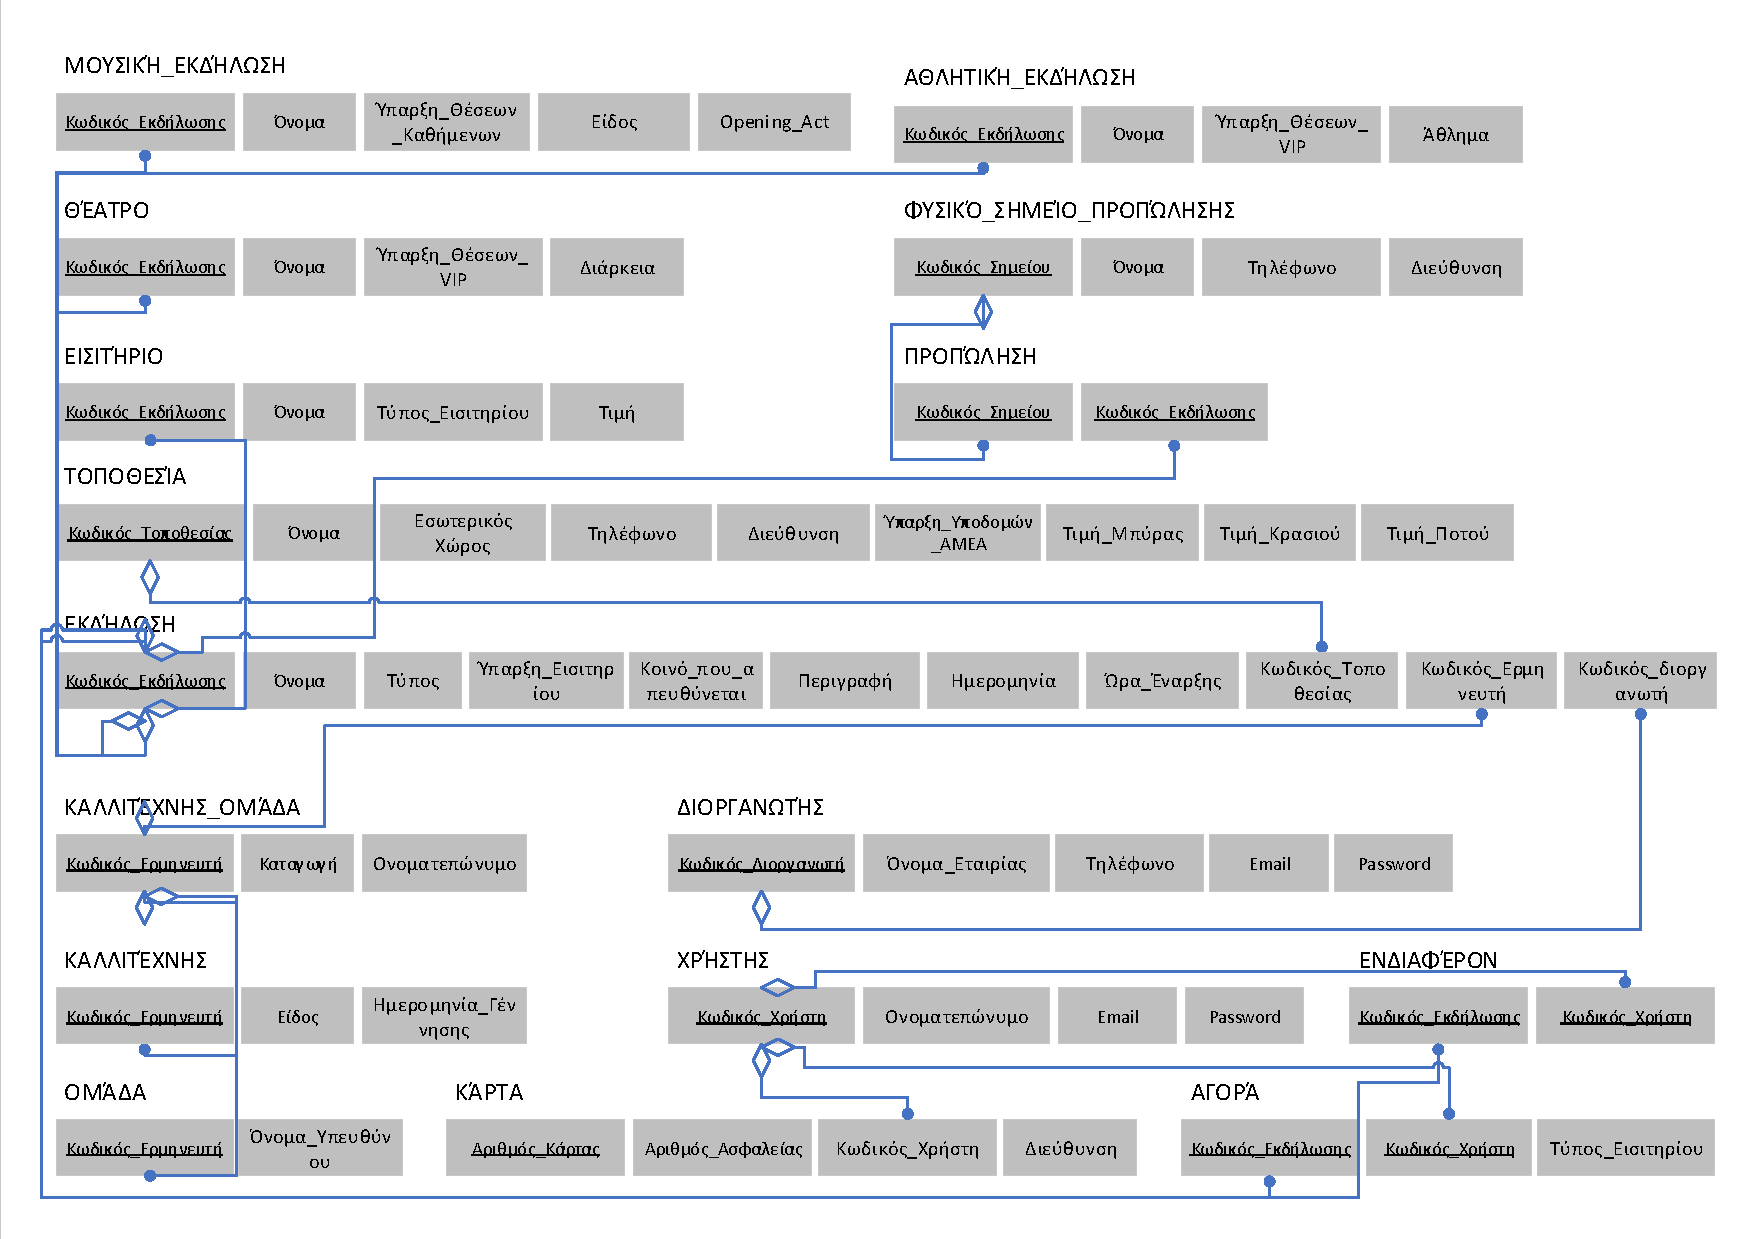
\includegraphics[width=\linewidth]{Relational.pdf}
  \caption{Σχεσιακό μοντέλο}
\end{figure}

\subsection{Όψεις}

Παρακάτω παρουσιάζονται κάποιες ενδεικτικές όψεις της βάσης δεδομένων
οι οποίες δίνουν μια πολύ καλή εικόνα για το πως όλες οι σχέσεις
συνδέονται μεταξύ τους. Αρκετές όψεις έχουν πολλές ομοιότητες μεταξύ
τους και γι' αυτόν τον λόγο θα παρουσιαστούν ενδεικτικά κάποιες από
αυτές.

Η κυριότερες όψεις αφορούν την προβολή στοιχείων εκδηλώσεων με διάφορα
κριτήρια. Οποιοσδήποτε συνδυασμός γνωρισμάτων μπορεί να προβληθεί στο
τέλος όμως στην παρακάτω περίπτωση θα προβληθεί μόνο το όνομα της
εκδήλωσης, η ημερομηνία και είτε το όνομα του καταστήματος διεξαγωγής
είτε το όνομα του καλλιτέχνη. Κάποια κριτήρια αναζήτησής εκδηλώσεων
είναι βάση του ονόματος του καταστήματος (\ref{eq1}), όνομα του
καλλιτέχνη (\ref{eq2}), ή συγκεκριμένου τύπου εκδήλωσης (\ref{eq3}).

\begin{equation} \label{eq1}
\begin{split}
&A \leftarrow \text{Εκδήλωση} \bowtie
\text{Καλλιτέχνης-Ομάδα} \bowtie
\sigma_{<\text{Όνομα\_τοποθεσίας} = \text{"Τα Ξύδια"}>}
\text{Τοποθεσία}
\\
&\Pi_{<\text{Όνομα\_εκδήλωσης, Ημερομηνία,Ονοματεπώνυμο}>}A
\end{split}
\end{equation}

\begin{equation} \label{eq2}
\begin{split}
&A \leftarrow \text{Εκδήλωση} \bowtie
\text{Τοποθεσία} \bowtie
\sigma_{<\text{Ονοματεπώνυμο} = \text{"Γιάννης Μπουζούκης"}>}
\text{Καλλιτέχνης-Ομάδα}
\\
&\Pi_{<\text{Όνομα\_εκδήλωσης, Ημερομηνία,Όνομα\_Τοποθεσίας}>}A
\end{split}
\end{equation}

\begin{equation} \label{eq3}
\begin{split}
&A \leftarrow \text{Καλλιτέχνης-Ομάδα} \bowtie
\sigma_{<\text{Τύπος} = \text{"Μουσική εκδήλωση"}>}\text{Εκδήλωση}
\\
&\Pi_{<\text{Όνομα\_εκδήλωσης, Ημερομηνία, Ονοματεπώνυμο}>}A
\end{split}
\end{equation}

Μία εξίσου σημαντική όψη είναι η αναζήτηση μια εκδήλωσης βάση της
ημέρας διεξαγωγής. Είτε για μία συγκεκριμένη ημερομηνία και ώρα είτε
για ένα εύρος (\ref{eq4}).

\begin{equation}
  \label{eq4}
  \begin{split}
    &\Pi_{<\text{Όνομα\_εκδήλωσης, Ημερομηνία, Ονοματεπώνυμο}>}(
    \sigma_{<\text{Ημερομηνία} = 23/11/2018>} \text{Εκδήλωση} \bowtie
    \text{Καλλιτέχνης-Ομάδα})
  \end{split}
\end{equation}

Πέρα από τις όψεις των εκδηλώσεων, μία σημαντική όψη αναγκαία για την
ολοκληρωμένη παροχή της υπηρεσίας αγοράς εισιτήριων είναι η προβολή
όλων των χρηστών όπου έχουν πραγματοποιήσει αγορά κάποιου εισιτηρίου
για μια συγκεκριμένη εκδήλωση (\ref{eq5}). Αυτή η όψη θα είναι διαθέσιμη μόνο στον
χρήστη Διοργανωτής ο οποίος συσχετίζεται με την εκάστοτε εκδήλωση.

\begin{equation}
  \label{eq5}
  \begin{split}
    &\Pi_{<\text{Ονοματεπώνυμο, Τύπος\_εισιτηρίου}>}(
    \sigma_{<\text{Κωδικός\_εκδήλωσης} = 42>} \text{Αγορά} \bowtie
    \text{Χρήστης})
  \end{split}
\end{equation}

Τέλος, μία ακόμα χρήσιμη όψη αφορά τον χρήστη Εγγεγραμμένος Χρήστης ο
οποίος θα θελήσει να προβάλει όλες τις αποθηκευμένες εκδηλώσεις όπου
έχει εκδηλώσει ενδιαφέρων (\ref{eq6}).


\begin{equation}
  \label{eq6}
  \begin{split}
    &A \leftarrow \sigma_{<\text{Κωδικός\_χρήστη} = 8055>}
    \text{Ενδιαφέρον} \bowtie \text{Εκδήλωση} \bowtie \text{Τοποθεσία}
    \bowtie \text{Καλλιτέχνης-Ομάδα} \\
    &\Pi_{<\text{Όνομα, Ημερομηνία, Ώρα\_έναρξης, Όνομα\_τοποθεσίας,
        Ονοματεπώνυμο}>}A
  \end{split}
\end{equation}


%%% Local Variables:
%%% mode: latex
%%% TeX-master: "main"
%%% TeX-engine: xetex
%%% End:
